%% Author_tex.tex
%% V1.0
%% 2012/13/12
%% developed by Techset
%%
%% This file describes the coding for modeloUFCG.cls

\documentclass[a4paper]{modeloUFCG} %%%% where modeloUFCG is the template name

\usepackage[portuguese]{babel}
\usepackage[T1]{fontenc}
\usepackage[utf8]{inputenc}
\usepackage{fancyhdr}
\usepackage{booktabs}
\usepackage{longtable}
\usepackage{array}
\usepackage{calc}
%% Fixa cada figura exatamente onde e gerada ([H]). Sem isso, floats podem
%% "flutuar" livremente e, neste documento (muitas figuras grandes em
%% sequencia), acabam se deslocando para muito longe do texto que os
%% referencia -- inclusive interferindo na quebra de pagina de tabelas
%% longtable vizinhas.
\usepackage{float}

%% A classe modeloUFCG.cls calcula largura/altura de texto e margens
%% assumindo o formato de trim de um periodico (174mm x 247mm), mas o PDF
%% final e produzido em A4 (210mm x 297mm). Isso deixa sobras enormes nas
%% margens. O pacote geometry forca margens A4 corretas, sobrepondo o
%% calculo original da classe.
\usepackage[a4paper, margin=2.5cm]{geometry}

\pagestyle{fancy}
\renewcommand{\headrulewidth}{0pt}
\fancyhead[L]{}
\fancyhead[C]{}
\fancyhead[R]{}

%% A classe usa \flushbottom, que estica os espacos em branco de cada pagina
%% para preenche-la ate o final. Combinado com figuras fixas ([H]), isso cria
%% buracos enormes entre uma figura/tabela e o texto seguinte. \raggedbottom
%% deixa o espaco sobrando apenas no rodape da pagina, sem esticar o meio.
\raggedbottom

%% Espacamento mais enxuto ao redor de figuras e tabelas.
\setlength{\floatsep}{8pt plus 2pt minus 2pt}
\setlength{\textfloatsep}{10pt plus 2pt minus 2pt}
\setlength{\intextsep}{8pt plus 2pt minus 2pt}


%%%% *** Do not adjust lengths that control margins, column widths, etc. ***

%%%%%%%%%%% Defining Enunciations  %%%%%%%%%%%
\newtheorem{theorem}{\bf Teorema}[section]
\newtheorem{condition}{\bf Condição}[section]
\newtheorem{corollary}{\bf Corolário}[section]
%%%%%%%%%%%%%%%%%%%%%%%%%%%%%%%%%%%%%%%%%%%%%%%

\usepackage{titlesec}
\renewcommand{\thesection}{\arabic{section}}
\renewcommand{\thesubsection}{\thesection.\arabic{subsection}}
\renewcommand{\thesubsubsection}{\thesubsection.\arabic{subsubsection}}

%%%% Cabecalho no estilo de artigo academico, substituindo a capa           %%%%
%%%% original (logo + caixa de titulo) do template Royal Society.          %%%%
%%%% A caixa de resumo estreita e trocada por um resumo de largura total,  %%%%
%%%% exibido logo apos o titulo/autores, como em um artigo convencional.   %%%%
%% Apos o \documentclass terminar de carregar, o LaTeX restaura o catcode de
%% @ para "outro", entao qualquer referencia a comandos internos da classe
%% (\@title, \@author, \if@subject@provided etc.) precisa ficar dentro de
%% \makeatletter ... \makeatother para ser reconhecida corretamente.
\makeatletter

%% Centraliza as legendas de figuras e tabelas (a classe original as deixa
%% alinhadas a esquerda).
\long\def\@makecaption#1#2{%
  \vskip\abovecaptionskip
  \centering{\captionheadfont #1.}\hskip2.5pt{\captionfont #2}\par
  \vskip\belowcaptionskip}

\renewenvironment{abstract}{%
  \global\setbox\absbox\vbox\bgroup\par\abstractfont
  \leftskip0pc\rightskip0pc\noindent\ignorespaces
}{\par\egroup}

%% A classe modeloUFCG.cls define \@maketitle atraves de mecanismos internos
%% (fila de duas colunas / bloco de revisao editorial) que absorvem qualquer
%% redefinicao de \@maketitle sem executa-la. Para evitar essa maquinaria,
%% \maketitle e redefinido diretamente aqui.
\renewcommand\maketitle{%
  \vspace*{-2.2cm}
  \noindent\begin{minipage}[c]{2.2cm}
    
\includegraphics[width=2cm]{lea_logo_bw}
  \end{minipage}%
  \begin{minipage}[c]{\textwidth-2.2cm}
    {\fontfamily{\sfdefault}\fontseries{b}\fontshape{n}\fontsize{12}{14}\selectfont
      UNIVERSIDADE FEDERAL DE CAMPINA GRANDE\par}
          {\fontfamily{\sfdefault}\fontseries{m}\fontshape{n}\fontsize{11}{13}\selectfont
       Disciplina: Estatística Aplicada%
        \quad---\quad Período: 2026.1\par}
              {\fontfamily{\sfdefault}\fontseries{m}\fontshape{n}\fontsize{11}{13}\selectfont
       Professores: Profa. Dra. Amanda Gomes; Prof.~Dr.~Jerfson Bruno; Prof.~Dr.~Gilberto Matos\par}
      \end{minipage}
  \vskip4pt
  \rule{\textwidth}{.5pt}
  \vskip8pt
  \begin{center}
    {\fontfamily{\sfdefault}\fontseries{m}\fontshape{n}\fontsize{16}{18}\selectfont\mathversion{bold}\@title\par}
    \vskip6pt
    {\authorfont\@author\par}
    \vskip3pt
    \ifx\@address\empty\else
      {\addressfont\@address\par}
    \fi
    \vskip6pt
    \rule{\textwidth}{.5pt}
  \end{center}
  \vskip8pt
  \ifvoid\absbox\else
    {\fontfamily{\sfdefault}\fontseries{b}\fontshape{n}\fontsize{11}{13}\selectfont Resumo}\par
    \vskip4pt
    \noindent\usebox\absbox\par
    \vskip6pt
  \fi
  \if@subject@provided
    {\subjectfont\@subject\par}
    \vskip4pt
  \fi
  \if@keywords@provided
    {\keywordfont\@keywords\par}
  \fi
  \vskip10pt
}

\makeatother

\begin{document}

%%%% Article title to be placed here
\title{Estatísticas de criminalidade violenta por estado americano (por 100 mil habitantes): assassinatos, assaltos e estupros, além do percentual da população urbana.}

\author{
Stefany Nicole Santos Alves$^{a}$}

\address{
  $^{a}$Departamento de Ciência da Computação - UFCG}
%%%% Subject entries to be placed here %%%%
\subject{
estatistica aplicada,
modelagem preditiva}

%%%% Keyword entries to be placed here %%%%
\keywords{
regressao linear multipla,
multicolinearidade,
selecao de modelos,
criminalidade,
diagnostico de residuos}

%%%% Abstract text to be placed here %%%%%%%%%%%%
\begin{abstract}
Este trabalho aplica a metodologia de regressão linear múltipla (MRLM) ao clássico conjunto de dados Iris, coletado por Anderson e popularizado por Fisher,
com o objetivo de modelar o comprimento da sépala a partir das demais variáveis morfológicas e da espécie da flor. Após uma análise exploratória uni e bivariada,
incluindo correlações, box-plots e verificação de dados ausentes, ajustamos um modelo inicial com todas as variáveis morfológicas contínuas e identificamos
multicolinearidade severa entre o comprimento e a largura da pétala. Comparamos modelos candidatos por AIC, BIC e teste F, selecionamos um modelo final e verificamos
seus pressupostos através de análise de resíduos, gráfico de envelope simulado e identificação de pontos atípicos, de alavanca e influentes. Em seguida, incorporamos
a espécie como variável qualitativa (dummy), discutindo a codificação por categoria de referência e o efeito de sua alteração sobre a interpretação dos coeficientes.
Por fim, para dois conjuntos de valores das variáveis explicativas, apresentamos os intervalos de confiança para o valor médio esperado da variável resposta e os
intervalos de predição para novas observações, com interpretação prática de ambos.
\end{abstract}
%%%%%%%%%%%%%%%%%%%%%%%%%%%

%% Some pieces required from the pandoc template
\providecommand{\tightlist}{%
  \setlength{\itemsep}{0pt}\setlength{\parskip}{0pt}}
\providecommand{\EndFirstPage}{%
}

\maketitle

\section{Introdução}\label{introduuxe7uxe3o}

A criminalidade é um tema importante para a análise de dados, pois diferentes fatores podem estar relacionados aos índices de violência. A base de dados utilizada
neste trabalho, \textbf{USArrests}, reúne informações dos 50 estados americanos referentes ao ano de 1973. Ela contém o número de \textbf{prisões por assassinato} (\texttt{Murder}),
\textbf{assalto} (\texttt{Assault}) e \textbf{estupro} (\texttt{Rape}), por 100 mil habitantes, além do percentual da população que vive em áreas urbanas (\texttt{UrbanPop}).

Neste trabalho, o objetivo é modelar o número de \textbf{prisões por assalto} (\texttt{Assault}) a partir das demais variáveis da base. Esse problema é interessante porque permite
analisar como diferentes tipos de crimes e o nível de urbanização estão relacionados com a variável resposta, além de aplicar técnicas de regressão linear múltipla.

Especificamente, buscamos:
(i) descrever a base de dados e realizar uma análise exploratória;
(ii) ajustar um modelo inicial de regressão linear múltipla;
(iii) avaliar a presença de multicolinearidade e selecionar um modelo mais adequado;
(iv) verificar os pressupostos do modelo; e
(v) interpretar os resultados obtidos.

\section{Metodologia}\label{metodologia}

Os dados correspondem aos 50 estados americanos no ano de 1973, sem valores ausentes, contendo quatro variáveis numéricas: \texttt{Murder}, \texttt{Assault}, \texttt{UrbanPop} e \texttt{Rape}.
A análise exploratória compreendeu estatísticas descritivas, matriz de correlação, histogramas, boxplots e matriz de dispersão entre as variáveis.

\subsection{Modelo de regressão linear múltipla}\label{modelo-de-regressuxe3o-linear-muxfaltipla}

Seja \(y_i\) o número de \textbf{prisões por assalto} da \(i\)-ésima observação (estado). O modelo inicial, utilizando todas as demais variáveis da base como explicativas, é dado por

\[
y_i = \beta_0 + \beta_1,\text{Murder}_i + \beta_2,\text{UrbanPop}_i + \beta_3,\text{Rape}_i + \varepsilon_i,
\]

\noindent em que \(\varepsilon_i\) segue as suposições usuais do Modelo de Regressão Linear Múltipla (MRLM) \cite{Kutner2004}: média nula, variância constante,
independência e normalidade.

A multicolinearidade entre as variáveis explicativas foi avaliada por dois critérios complementares: (a) a matriz de correlações entre as variáveis preditoras,
em que valores absolutos de correlação maiores que 0,8 indicam possível multicolinearidade; e (b) o fator de inflação da variância (VIF), dado por
\(\text{VIF}_j = 1/(1-R_j^2)\), em que \(R_j^2\) é o coeficiente de determinação da regressão de \(X_j\) sobre as demais variáveis explicativas. Valores de \(\text{VIF}\)
superiores a 5 indicam possível problema de multicolinearidade, enquanto valores acima de 10 sugerem multicolinearidade severa \cite{Kutner2004}.

A seleção do modelo foi realizada utilizando os critérios de informação de Akaike (AIC) \cite{Akaike1974} e Bayesiano (BIC) \cite{Schwarz1978}, além do teste
\(F\) para comparação entre modelos aninhados. Em ambos os critérios de informação, modelos com menores valores de AIC e BIC são preferíveis. Como apoio à seleção,
também foi utilizado o procedimento automático \emph{stepwise} (\texttt{step}), baseado no critério AIC, permitindo comparar a seleção automática com a escolha baseada na interpretação
estatística dos resultados.

\subsection{Diagnóstico do modelo}\label{diagnuxf3stico-do-modelo}

A adequação do modelo selecionado foi avaliada por meio da análise gráfica dos resíduos, utilizando os gráficos de resíduos versus valores ajustados, quantil-quantil
(Q-Q Plot), escala-localização e resíduos versus alavancagem. Esses gráficos permitem verificar os principais pressupostos do Modelo de Regressão Linear Múltipla,
como linearidade, homocedasticidade, normalidade dos resíduos e a presença de observações influentes \cite{Kutner2004}.

Também foram analisadas possíveis observações atípicas, de alavanca e influentes utilizando os resíduos studentizados (\(|t_i| > 2\)), os valores de alavancagem
(\(h_{ii} > 2p/n\)) e a distância de Cook (\(D_i > 4/n\)) \cite{Cook1977,CookWeisberg1982,Kutner2004}. Caso fossem identificadas observações com influência significativa
sobre o ajuste, seria avaliado o impacto de sua remoção por meio do reajuste do modelo.

Por fim, para facilitar a comparação da influência das variáveis explicativas, foram calculados os coeficientes padronizados do modelo final. Como as variáveis estão em
escalas diferentes, essa padronização permite comparar diretamente a contribuição relativa de cada variável para explicar o número de prisões por assalto.

\subsection{Variáveis explicativas}\label{variuxe1veis-explicativas}

Diferentemente de outros conjuntos de dados que possuem variáveis categóricas, a base \textbf{USArrests} é composta apenas por variáveis numéricas (\texttt{Murder}, \texttt{UrbanPop} e \texttt{Rape}),
utilizadas como variáveis explicativas do modelo. Dessa forma, não foi necessária a criação de variáveis \emph{dummy} nem a definição de uma categoria de referência.
O modelo foi ajustado diretamente utilizando essas variáveis contínuas para explicar o número de prisões por assalto (\texttt{Assault}).

\subsection{Inferência preditiva}\label{inferuxeancia-preditiva}

Para um conjunto de valores das variáveis explicativas (\texttt{Murder}, \texttt{UrbanPop} e \texttt{Rape}), é possível realizar dois tipos de inferência \cite{Kutner2004}:
o \textbf{intervalo de confiança} para o valor médio esperado de prisões por assalto, que estima a média da resposta para estados com essas características, e
o \textbf{intervalo de predição} para uma \textbf{nova observação}, que estima um valor futuro de prisões por assalto para um estado com as mesmas características.
Como o intervalo de predição considera também a variabilidade entre observações individuais, ele é naturalmente mais amplo que o intervalo de confiança.
Ambos foram calculados para dois conjuntos hipotéticos de valores das variáveis explicativas, escolhidos dentro do intervalo observado na base de dados.

\section{Resultados}\label{resultados}

\subsection{Descrição da base de dados}\label{descriuxe7uxe3o-da-base-de-dados}

A base \texttt{USArrests} possui \(n = 50\) observações, correspondentes aos 50 estados americanos, e 4 variáveis numéricas (Tabela \ref{tab:variaveis}), sem valores ausentes.

\begin{longtable}[]{@{}
  >{\raggedright\arraybackslash}p{(\linewidth - 4\tabcolsep) * \real{0.0900}}
  >{\raggedright\arraybackslash}p{(\linewidth - 4\tabcolsep) * \real{0.6400}}
  >{\raggedright\arraybackslash}p{(\linewidth - 4\tabcolsep) * \real{0.2700}}@{}}
\caption{\label{tab:variaveis} Variáveis da base de dados \protect\texttt{USArrests}, descrição e unidade de medida.}\tabularnewline
\toprule\noalign{}
\begin{minipage}[b]{\linewidth}\raggedright
Variável
\end{minipage} & \begin{minipage}[b]{\linewidth}\raggedright
Descrição
\end{minipage} & \begin{minipage}[b]{\linewidth}\raggedright
Unidade
\end{minipage} \\
\midrule\noalign{}
\endfirsthead
\toprule\noalign{}
\begin{minipage}[b]{\linewidth}\raggedright
Variável
\end{minipage} & \begin{minipage}[b]{\linewidth}\raggedright
Descrição
\end{minipage} & \begin{minipage}[b]{\linewidth}\raggedright
Unidade
\end{minipage} \\
\midrule\noalign{}
\endhead
\bottomrule\noalign{}
\endlastfoot
Murder & Prisões por assassinato (por 100 mil habitantes) & prisões/100 mil habitantes \\
Assault & Prisões por assalto (variável resposta, por 100 mil habitantes) & prisões/100 mil habitantes \\
UrbanPop & Percentual da população urbana & \% \\
Rape & Prisões por estupro (por 100 mil habitantes) & prisões/100 mil habitantes \\
\end{longtable}

\subsection{Análise exploratória}\label{anuxe1lise-exploratuxf3ria}

A Tabela \ref{tab:descritivas} apresenta as estatísticas descritivas das variáveis da base \texttt{USArrests}.

\begin{longtable}[]{@{}llrr@{}}
\caption{\label{tab:descritivas}\label{tab:descritivas} Média e desvio-padrão (dp) das variáveis da base USArrests.}\tabularnewline
\toprule\noalign{}
& Variável & Média & Desvio.padrão \\
\midrule\noalign{}
\endfirsthead
\toprule\noalign{}
& Variável & Média & Desvio.padrão \\
\midrule\noalign{}
\endhead
\bottomrule\noalign{}
\endlastfoot
Murder & Murder & 7.79 & 4.36 \\
Assault & Assault & 170.76 & 83.34 \\
UrbanPop & UrbanPop & 65.54 & 14.47 \\
Rape & Rape & 21.23 & 9.37 \\
\end{longtable}

A Figura \ref{fig:boxplots} apresenta os box-plots das variáveis da base. Observa-se que \texttt{Assault} e \texttt{Rape} apresentam maior dispersão dos dados, enquanto \texttt{UrbanPop} possui distribuição mais concentrada. Além disso, algumas variáveis apresentam observações mais afastadas da maior parte dos dados, indicando possíveis valores extremos.

\begin{figure}[H]

{\centering 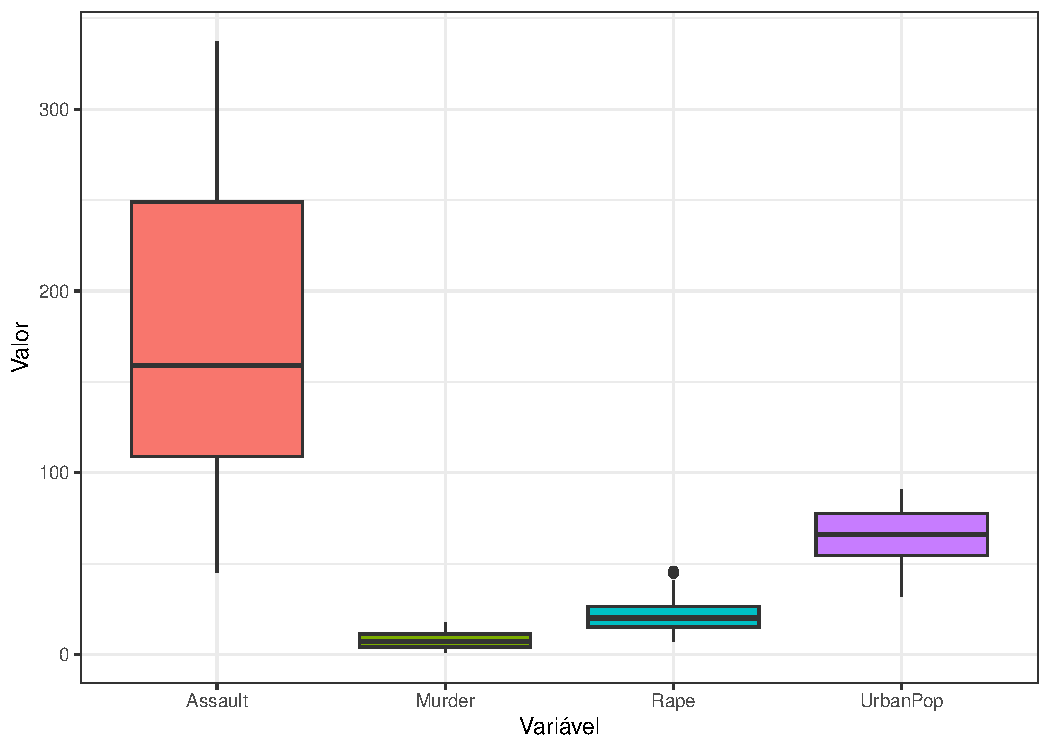
\includegraphics[width=1\linewidth]{relatorio_files/figure-latex/boxplots-1} 

}

\caption{\label{fig:boxplots} Box-plots das variáveis da base USArrests.}\label{fig:boxplots}
\end{figure}

\subsubsection{Análise de correlação}\label{anuxe1lise-de-correlauxe7uxe3o}

A Figura \ref{fig:corrplot} apresenta a matriz de correlações entre as quatro variáveis da base.

\begin{figure}[H]

{\centering 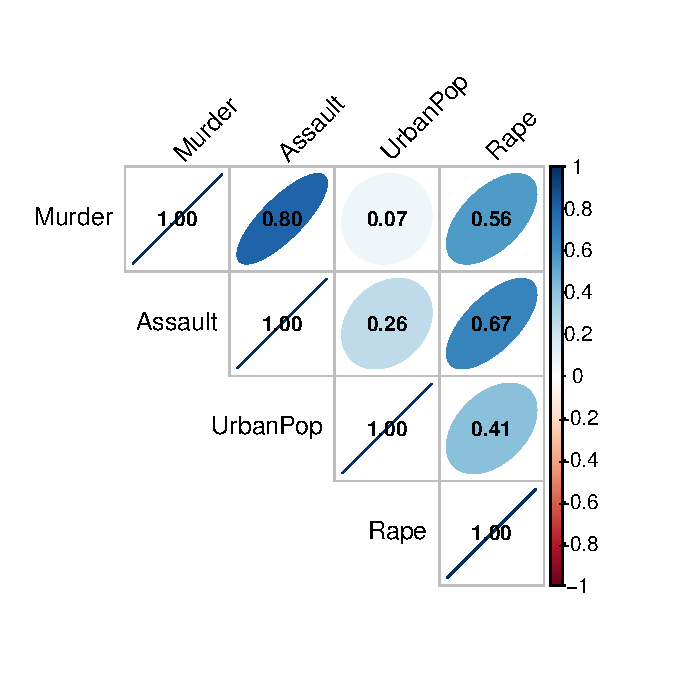
\includegraphics[width=0.65\linewidth]{relatorio_files/figure-latex/corrplot-1} 

}

\caption{\label{fig:corrplot} Matriz de correlações entre as variáveis da base USArrests.}\label{fig:corrplot}
\end{figure}

Com relação à análise de correlação, espera-se que as variáveis explicativas apresentem correlação com a variável resposta \texttt{Assault}, mas que as correlações entre as próprias variáveis explicativas não sejam excessivamente elevadas, pois isso pode indicar multicolinearidade. Como regra geral, correlações absolutas superiores a 0,8 merecem atenção.

Examinando a Figura \ref{fig:corrplot}, observa-se que:

\begin{enumerate}
\def\labelenumi{\arabic{enumi}.}
\item
  A variável resposta \texttt{Assault} apresenta correlação positiva com \texttt{Murder} e \texttt{Rape}, indicando que estados com maiores índices de prisões por assassinato e estupro tendem também a apresentar maiores índices de prisões por assalto.
\item
  A variável \texttt{UrbanPop} apresenta correlação mais fraca com as demais variáveis, sugerindo menor associação linear com os índices de criminalidade.
\item
  As correlações entre as variáveis explicativas (\texttt{Murder}, \texttt{UrbanPop} e \texttt{Rape}) serão avaliadas juntamente com o VIF para verificar a existência de multicolinearidade.
\end{enumerate}

\subsubsection{Multicolinearidade: o VIF}\label{multicolinearidade-o-vif}

Para quantificar a multicolinearidade sugerida pela análise de correlação, ajustamos um modelo inicial considerando \texttt{Assault} como variável resposta e \texttt{Murder}, \texttt{UrbanPop} e \texttt{Rape} como variáveis explicativas.

\begin{longtable}[]{@{}lrrrr@{}}
\caption{\label{tab:coefInicial} Estimativas dos coeficientes do modelo inicial.}\tabularnewline
\toprule\noalign{}
Termo & Estimativa & Erro Padrão & Estatística t & p-valor \\
\midrule\noalign{}
\endfirsthead
\toprule\noalign{}
Termo & Estimativa & Erro Padrão & Estatística t & p-valor \\
\midrule\noalign{}
\endhead
\bottomrule\noalign{}
\endlastfoot
Intercepto & -15.4520 & 31.8581 & -0.4850 & 0.6300 \\
Murder & 12.4700 & 1.8533 & 6.7286 & 0.0000 \\
UrbanPop & 0.6304 & 0.5054 & 1.2474 & 0.2186 \\
Rape & 2.2502 & 0.9432 & 2.3857 & 0.0212 \\
\end{longtable}

\begin{longtable}[]{@{}lr@{}}
\caption{\label{tab:vifCompleto} Fator de inflação de variância (VIF) das variáveis explicativas.}\tabularnewline
\toprule\noalign{}
Variável & VIF \\
\midrule\noalign{}
\endfirsthead
\toprule\noalign{}
Variável & VIF \\
\midrule\noalign{}
\endhead
\bottomrule\noalign{}
\endlastfoot
Murder & 1.54 \\
UrbanPop & 1.26 \\
Rape & 1.84 \\
\end{longtable}

O modelo inicial será avaliado por meio do coeficiente de determinação ajustado, da significância dos coeficientes e dos valores de VIF. Valores de VIF superiores a 5 indicam possível multicolinearidade, enquanto valores acima de 10 caracterizam um problema mais severo. Caso seja identificada multicolinearidade relevante, será realizada a seleção de um modelo mais adequado antes da análise dos pressupostos.

\subsection{Seleção do modelo final}\label{seleuxe7uxe3o-do-modelo-final}

\subsubsection{\texorpdfstring{Seleção automática via \texttt{step}}{Seleção automática via step}}\label{seleuxe7uxe3o-automuxe1tica-via-step}

\subsection{Diagnóstico do modelo selecionado}\label{diagnuxf3stico-do-modelo-selecionado}

\subsubsection{Identificação de pontos atípicos, de alavanca e influentes}\label{identificauxe7uxe3o-de-pontos-atuxedpicos-de-alavanca-e-influentes}

\subsubsection{Impacto da remoção dos pontos influentes}\label{impacto-da-remouxe7uxe3o-dos-pontos-influentes}

\subsection{Interpretações do modelo selecionado}\label{interpretauxe7uxf5es-do-modelo-selecionado}

\subsubsection{Coeficientes padronizados}\label{coeficientes-padronizados}

\subsection{Regressão com variáveis dummy (a espécie como explicativa)}\label{regressuxe3o-com-variuxe1veis-dummy-a-espuxe9cie-como-explicativa}

\subsubsection{\texorpdfstring{Modelo sem \texttt{Petal.Length}, com a espécie}{Modelo sem Petal.Length, com a espécie}}\label{modelo-sem-petal.length-com-a-espuxe9cie}

\subsubsection{Alterando a categoria de referência}\label{alterando-a-categoria-de-referuxeancia}

\subsection{Comparação geral dos modelos}\label{comparauxe7uxe3o-geral-dos-modelos}

\section{Previsões}\label{previsuxf5es}

\subsection{Intervalo de confiança para o valor médio esperado}\label{intervalo-de-confianuxe7a-para-o-valor-muxe9dio-esperado}

\subsection{Intervalo de predição para uma nova observação}\label{intervalo-de-prediuxe7uxe3o-para-uma-nova-observauxe7uxe3o}







\bibliographystyle{RS}
\bibliography{modeloUFCG.bib}


\end{document}
